\documentclass{article}
% Packages
\usepackage{graphicx,subfig,float} % Required for inserting images
\usepackage{amsmath}
\usepackage{datetime}
\usepackage[spanish]{babel}
\usepackage{titling}
\usepackage{geometry}
\usepackage{tabularray}

\geometry{
  a4paper,
  total={170mm,257mm},
  width=150mm,
  height=230mm,
}

\usepackage{tcolorbox}

\graphicspath{{assets/}}

\numberwithin{equation}{section}
\renewcommand{\theequation}{\arabic{section}.\arabic{equation}}

\newenvironment{subs}
  {\adjustwidth{3em}{0pt}}
  {\endadjustwidth}

\providecommand{\abs}[1]{\lvert#1\rvert}


\title{Módulo 2 \\ Conceptos de Arquitectura de Computadoras}
\author{Polanis, Iván Valentín}
\date{}

\begin{document}

\maketitle

\newpage
\tableofcontents
\newpage

\section{Segmentación de instrucciones}

En una arquitectura \textbf{RISC}\footnote{Reduced Instruction Set Computer} la mayoría de las instrucciones son del tipo registro a registro, y un ciclo de instrucción tiene las dos fases siguientes:

\begin{itemize}
  \item \textbf{I}: captación de instrucción
  \item \textbf{E}: ejecución. Realiza una operación de la ALU como entrada y salida.
\end{itemize}

Las operaciones de carga y almacenamiento necesitan tres fases:

\begin{itemize}
  \item \textbf{I}: captación de instrucción
  \item \textbf{E}: ejecución. Calcula una dirección de memoria.
  \item \textbf{D}: memoria. Operación registro a memoria o memoria a registro.
\end{itemize}

Dada la simplicidad y regularidad de un repertorio de instrucciones RISC, el diseño de la organización en tres o cuatro etapas se realiza fácilmente. 

\subsection{Optimización de la segmentación}

Dada la naturaleza sencilla y regular de las instrucciones RISC, los esquemas de segmentación se pueden emplear eficientemente. Hay poca variación en la duración de la ejecución de instrucciones, y el cauce puede adaptarse para reflejar este hecho.

Para compensar las dependencias de datos, se han desarrollado técnicas de reorganización de código. Consideremos primero las instrucciones de salto. El \textit{salto retardado}, que es una forma de incrementar la eficiencia de la segmentación, utiliza un salto que no tiene lugar hasta después de que se ejecute la siguiente instrucción. La posición de la instrucción inmediatamente después de la instrucción de salto se conoce como \textit{espacio de retardo}.

Para saltos condicionales, el procedimiento no puede aplicarse a ciegas. Si la condición comprobada por la bifurcación puede alterarse por la instrucción inmediatamente precedente, el compilador ha de abstenerse de hacer el intercambio en su lugar, debe inserta un NOOP.

Un tipo de táctica similar, llamada \textit{carga retardada}, se puede usar con las instrucciones LOAD. En las instrucciones LOAD, el procesador bloquea el registro destino de la carga. Después el procesador continúa la ejecución del flujo de instrucciones hasta que se alcanza una instrucción que necesite ese registro, deteniéndose hasta que la carga finalice. Si el compilador puede reorganizar las instrucciones de manera que se pueda hacer un trabajo útil mientras la carga está en el cauce, la eficiencia aumenta.


\section{Soluciones a Atascos}

\subsection{Soluciones a riesgos estructurales}

La solución es simple, se debe replicar, segmentar o realizar turnos para el acceso a las unidades funcionales en conflicto.

\begin{itemize}
  \item Duplicación de recursos de hardware.
  \subitem{Sumadores o restadores además de la ALU.}
  \item Separación en memorias de instrucciones y datos.
  \item Turnar el acceso al banco de registro.
  \subitem{Escrituras en la primera mitad del ciclo de reloj.}
  \subitem{Lecturas en la segunda mitad del ciclo de reloj.}
\end{itemize}

\subsection{Soluciones a riesgos de datos}

Para riesgos \textbf{RAW} se debe determinar cómo y cuando aparecen esos riesgos. Para ello será necesario una unidad de detección de riesgos y/o un compilador más complejo.

Para este tipo de riesgo tenemos dos soluciones:

\begin{itemize}
  \item \textbf{Hardware}
  \subitem{Adelantamiento de operandos (Forwarding).}
  \item \textbf{Software}
  \subitem{Instrucciones NOP o reordenamiento de de codigo.}
\end{itemize}

\subsubsection{Adelantamiento de operandos (Forwarding)}

Esta técnica consiste en pasar directamente el resultado obtenido con una instrucción a las instrucciones que lo necesitan como operando. Si el dato necesario está disponible a la salida de la ALU ($X_i$) se lleva a la entrada de la etapa correspondiente ($X_{i+1}$) sin esperar a la escritura ($M_i$ o $W_i$).

\begin{figure}[H]
  \centering
  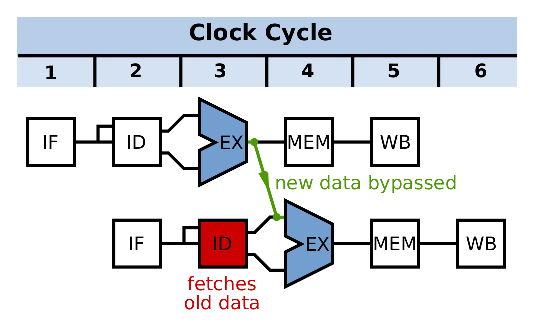
\includegraphics[width=0.7\textwidth]{Forwarding}
  \caption{Adelantamiento de operandos.} 
\end{figure}

\subsubsection{Instrucciones NOP o reordenamiento de código}

Evita los riesgos reordenando las instrucciones del código sin afectar el código. El compilador es el encargado de realizar esta tarea.

Aquí se introducen las instrucciones NOP, que son utilizadas para generar un retardo. Estas instrucciones no realizan ninguna operación, pero consumen un ciclo de reloj. Ademas, se reordenan instrucciones para evitar riesgos RAW.\@

\subsection{Soluciones a riesgos de control}

En los riesgos de control se introduce la penalización por salto. Cuando el salto es incondicional, la dirección de destino se debe determinar lo más pronto posible, dentro del cauce, para reducir la penalización. Cuando el salto es condicional, la penalización se debe a que el procesador no sabe si se debe tomar o no el salto hasta que se evalúe la condición.

Se utiliza una modificación sencilla de la ruta de datos para reducir la cantidad de paradas a un solo ciclo:

\begin{itemize}
  \item \textbf{Adelantar la resolución de los saltos a la etapa D}
  \begin{itemize}
    \item En ella se decodifica y se sabe que es un salto.
    \item Se puede evaluar la condición de salto.
    \item Se puede calcular la dirección de destino.
  \end{itemize}
\end{itemize}

\subsubsection{Técnicas de predicción de salto (Hardware)}

Para este tipo de técnicas tenemos dos posibilidades:

\begin{itemize}
  \item \textbf{Predicción estática}
  \subitem{Se asume que el salto se toma o no se toma.}
  \item \textbf{Predicción dinámica}
  \subitem{Se utiliza un predictor de saltos.}
\end{itemize}

\subsubsection*{Predicción estática}

\begin{itemize}
  \item \textbf{Predicción de salto tomado}
  \subitem{Se asume que el salto se toma.}
  \subitem{Se adelanta la búsqueda de la dirección de destino.}
  \item \textbf{Predicción de salto no tomado}
  \subitem{Se asume que el salto no se toma.}
  \subitem{Se continúa con la ejecución secuencial.}
\end{itemize}

\subsubsection*{Predicción dinámica}

\begin{itemize}
  \item \textbf{Conmutador saltar/no saltar}
  \begin{itemize}
    \item Basado en la historia de las instrucciones.
    \item Es eficaz para los bucles.
  \end{itemize}
  \item \textbf{Tabla de historia de saltos (BTB)}
  \begin{itemize}
    \item Pequeña cache asociada a la etapa de búsqueda (F).
    \item Contiene tres campos.
    \subitem{Dirección de una instrucción de bifurcación.}
    \subitem{Información de la instrucción destino.}
    \subitem{N bits de estado (histórico).}
  \end{itemize}
\end{itemize}

\subsubsection*{Otras soluciones}

Una técnica que se utiliza es la \textbf{predicción según el código de operación}, ya que existen instrucciones con más probabilidades de saltar. La tasa de acierto es del 75\%.

Los \textbf{Flujos múltiples} utilizan varios cauces (uno por cada opción de salto). Precaptan cada salto en diferentes cauces. Las desventajas son que provoca retardos en el acceso al bus y a los registros. Si hay múltiples saltos, se necesita un mayor número de cauces.

La \textbf{Precaptación del destino de salto} consiste en precaptar la instrucción destino del salto, además de las instrucciones siguientes a la bifurcación. La instrucción se guarda hasta que se ejecute la instrucción de bifurcación.

En el \textbf{Buffer de bucles} se utiliza una memoria muy rápida gestionada por la etapa de captación de instrucción del cauce. Comprueba el buffer antes de hacer la captación de memoria. Esta técnica es muy eficaz para pequeños bucles y saltos.

\subsubsection{Instrucciones de salto retardado (Software)}

La idea es realizar trabajo útil mientras el salto se resuelve.

\begin{itemize}
  \item Hueco o ranura de retardo de salto es el período de penalización o parada luego de una instrucción de salto.
  \item El compilador trata de situar instrucciones útiles (que no dependan del salto) en los huecos de retardo. Si no es posible, se utilizan instrucciones NOP.\@
  \item Las instrucciones en los huecos de retardo de salto se captan siempre.
  \item Requiere reordenamiento de código.
\end{itemize}
\section{Computadoras de repertorio reducido de instrucciones}

Algunos de los principales avances desde el nacimiento del computador son:

\begin{itemize}
  \item \textbf{El concepto de familia:} introducido por IBM en su System/360 em 1964. El concepto de familia separa la arquitectura de una máquina de su implementación. Se ofrece un conjunto de computadores, con distintas características en cuanto a precio/prestaciones, que presentan al usuario la misma arquitectura.
  \item \textbf{Unidad de control micro programada:} propuesta por Wilkes en 1951, e introducida por iBM en la línea S/360 en 1964. La micro programación facilita la tarea de diseñar e implementar la unidad de control y da soporte al concepto de familia.
  \item \textbf{Memoria caché:} introducida en 1968 por IBM.\@ La introducción de este elemento en la jerarquía de memoria mejoró las prestaciones de manera espectacular.
  \item \textbf{Segmentación de cauce:} una manera de introducir paralelismo en la naturaleza esencialmente secuencial de un por instrucciones máquina.
\end{itemize}

La arquitectura RISC se aparta de manera drástica de la tendencia histórica en la arquitectura del procesador. Un análisis de la arquitectura RISC involucra la mayoría de los asuntos importantes de organización y arquitectura de computadores.

Los sistemas RISC están caracterizados por:

\begin{itemize}
  \item Un gran número de registros de uso general, o el uso de tecnología de compiladores para optimizar la utilización de los registros.
  \item Un repertorio de instrucciones limitado y sencillo.
  \item Un énfasis en la optimización de la segmentación de instrucciones.
\end{itemize}

\subsection{Características de la ejecución de instrucciones}

Los repertorios complejos de instrucciones están pensados para:

\begin{itemize}
  \item Facilitar el trabajo del escritor de compiladores.
  \item Mejorar la eficiencia de la ejecución, ya que las secuencias complejas de operaciones pueden implementarse en micro código.
  \item Dar soporte a HLL\footnote{High Level Language} aun más complejos y sofisticados.
\end{itemize}

Para comprender la línea de razonamiento de los partidarios de los RISC, comenzamos con una breve revisión de las características de la ejecución de instrucciones. Los aspectos cuyo cálculo tiene interés son los siguientes:

\begin{itemize}
  \item \textbf{Operaciones realizadas:} determinan las funciones que lleva a cabo el procesador y su interacción con la memoria.
  \item \textbf{Operandos usados:} los tipos de operandos y su frecuencia de uso determinan la organización de memoria para almacenarlos y los modos de direccionamiento para acceder a ellos.
  \item \textbf{Secuenciamiento de la ejecución:} determina la organización del control y del cauce segmentado.
\end{itemize}

\subsubsection*{Operaciones}

Existe una gran concordancia en los resultados de esta mezcla de lenguajes y aplicaciones. Las sentencias de asignación predominan, lo cual indica que el sencillo movimiento de datos tiene mucha importancia. También predominan las sentencias condicionales (IF, LOOP). Estas sentencias se implementen en el lenguaje máquina con alguna instrucción del tipo comparar y saltar. Esto indica que el mecanismo incluido en el repertorio de instrucciones para el control del secuenciamiento es importante.

Estos resultados son instructivos para el diseñador del repertorio de instrucciones máquina, diciéndole qué tipo de sentencias tiene lugar más a menudo y por consiguiente deben ser implementadas de una forma óptima.

\subsubsection*{Operandos}

EL estudio de Patterson ya referenciado también consideró la frecuencia dinámica de aparición de distintas clases de variables. Los resultados, coherentes para programas en Pascal y en C, muestran que la mayoría de las referencias se hacen a variables escalares simples. Además, más del ochenta por ciento de los datos  eran variables locales. Asimismo, las referencias a matrices/estructuras requieren una referencia previa a su índice o puntero, que nuevamente suele ser un dato escalar local. Por consiguiente, hay un predominio de referencias a operandos escalares, y estos están muy localizados.

Estos estudios reflejan la importancia de una arquitectura que se preste a un rápido acceso a operandos, dado que es una operación que se realiza con mucha frecuencia. El estudio de Patterson indica que un candidato fundamental a optimizar es el mecanismo de almacenamiento y acceso a variables escalares.

\subsubsection*{Llamadas a procedimientos}

Las llamadas y retornos de procedimientos constituyen un aspecto importante de los programas en HLL.\@ Los estudios indican que son las operaciones que consumen más tiempo en programas en HLL compilados.

Esto depende del número de parámetros tratados y del nivel de anidamiento. La mayoría de los programas no tienen una larga secuencia de llamadas seguida por la correspondiente secuencia de retornos. Además la mayoría de las variables suelen ser locales y las referencias a operandos están muy localizadas.

Partiendo del trabajo de varios investigadores, surgen tres elementos que, por lo general, caracterizan las arquitecturas RISC:\@

\begin{itemize}
  \item \textbf{Utilización de un amplio banco de registros}
  \item \textbf{Cuidadosa atención al diseño de los cauces de instrucciones.}
  \item \textbf{Uso de un repertorio simplificado de instrucciones}
\end{itemize}

\subsection{Utilización de un amplio banco de registros}

Se necesita una estrategia que permita que los operandos a los que se acceda con mayor frecuencia se encuentren en registros y se minimicen las operaciones registro-memoria.

Son posibles dos aproximaciones básicas, una basada en software y la otra en hardware.

La aproximación por software consiste en confiar al compilador la maximización del uso de los registros. El compilador intentará asignar registros a las variables que se usen más en un periodo dado. Esta solución requiere el uso de sofisticados algoritmos de análisis de programas.

La aproximación por hardware consiste sencillamente en usar más registros de manera que puedan mantenerse en ellos más variables durante períodos de tiempo más largos.

\subsubsection*{Ventanas de registros}

A primera vista, el uso de un conjunto amplio de registros debería reducir la necesidad de acceder a memoria. La labor del diseño es organizar los registros de tal modo que se alcance esa meta.

Una llamada a un procedimiento hace que el procesador conmute automáticamente a una ventana de registros distinta de tamaño fijo, en lugar de salvaguardar los registros en memoria. Las ventanas de procedimientos adyacentes están parcialmente solapadas para permitir el paso de parámetros.

La ventana se divide en tres áreas de tamaño fijo. Los registros de parámetros contienen parámetros pasados al procedimiento actual desde el procedimiento que lo llamó, y los resultados a devolver a este. Los registros locales se usan para variables locales, según la asignación que realice el compilador. Los registros locales se usan para variables locales, según la asignación que realice el compilador. Los registros temporales se usan para intercambiar parámetros y resultados con el siguiente nivel más bajo (el procedimiento llamado por el procedimiento en curso). Los registros temporales de un nivel son físicamente los mismos que los registros de parámetros del nivel más bajo adyacente. Este solapamiento posibilita que los parámetros se pasen sin que exista una transferencia de datos real.

Para manejar cualquier patrón posible de llamadas y retornos, el número de ventanas de registros tendría que ser ilimitado. En lugar de eso, las ventanas de registros se pueden usar para contener unas pocas, las más recientes, activaciones de procedimientos. Las activaciones más antiguas han de salvaguardarse en memoria y restaurarse más tarde cuando la profundidad de anidamiento disminuya.

\begin{figure}[H]
  \centering
  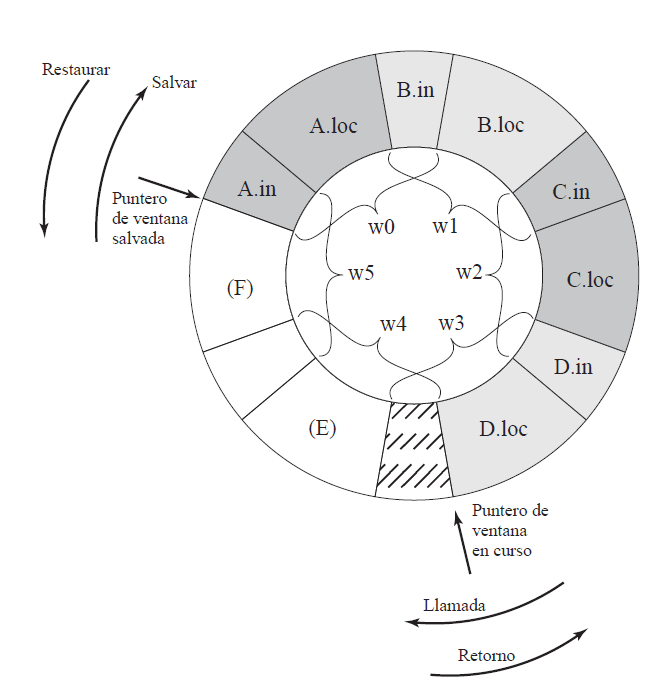
\includegraphics[width=0.5\textwidth]{Buffer.png}
  \caption{Organización de las ventanas solapadas con un buffer circular.}
\end{figure}

\subsubsection*{Variables Globales}

Para tratar variables globales se sugieren dos opciones.

La primera es que el compilador asigne posiciones de memoria a las variables declaradas como globales en un HLL, y que todas las instrucciones máquina que referencien esas variables declaradas como globales en un HLL, y que todas las instrucciones máquina que referencien esas variables usen operandos referenciados en memoria.

Una alternativa es incorporar al procesador un conjunto de registros globales. Estos registros serían fijos en cuanto a su número y accesibles por todos los procedimientos. Se puede usar un esquema de numeración unificado para simplificar el formato de instrucción. Esto conlleva un hardware añadido, que se encarga de adaptar la división en el direccionamiento de los registros.

\subsubsection*{Un amplio banco de registros frente a una caché}

\begin{table}[h]
  \centering
  \begin{tabular}{|l|l|}
    \cline{1-2}
    \multicolumn{1}{|c|}{\textbf{Banco de registros amplio}} & \multicolumn{1}{c|}{\textbf{Caché}} \\ \cline{1-2}
                                                             Todos los datos escalares locales & Datos escalares locales recientemente usados \\ \cline{1-2}
                                                             Variables individuales & Bloques de memoria \\ \cline{1-2}
                                                             Variables globales asignadas por el compilador & Variables recientemente \\ \cline{1-2}
                                                             Salvaguarda basadas en la profundidad de anidamiento & Salvaguarda basadas en el algoritmo de reemplazo \\ \cline{1-2}
                                                             Direccionamiento a registros & Direccionamiento a memoria \\ \cline{1-2}
  \end{tabular}
\end{table}

\subsection{Optimización de registros basada en el compilador}

Supongamos que ahora disponemos de una máquina RISC que contiene unicamente un pequeño número de registros. En ese caso, el uso optimizado de registros es responsabilidad del compilador. Los programas escritos en HLL no tienen referencias explicitas a los registros. El objetivo del compilador es mantener en registros en lugar de en memoria los operandos necesarios para tantos cálculos como sea posible, y minimizar las operaciones de carga y almacenamiento.

Por lo general se sigue el siguiente enfoque. Cada cantidad del programa candidata para residir en un registro se asigna a un registro simbólico o virtual. El compilador entonces asigna el número ilimitado de registros simbólicos a un número fijo de registros reales. Los registros simbólicos cuya utilización no se solape pueden compartir el mismo registro real. Si en una parte concreta del programa hay más cantidades a tratar que registros reales, algunas de las cantidades se asignan a posiciones de memoria.

\subsection{Arquitectura de repertorio reducido de instrucciones}

\subsubsection*{¿Por qué CISC?}

La primera de las razones es, la simplificación de los compiladores. La labor del escritor de compiladores es generar una secuencia de instrucciones máquina para cada sentencia HLL.\@ Se existen instrucciones máquina que se parezcan a sentencias del HLL, la tarea se simplifica.

La otra razón importante mencionada es la esperanza de que un CISC produzca programas más pequeños y rápido. Los programas más pequeños tienen dos ventajas. Como el programa ocupa menos memoria, hay un ahorro de este recurso, pero como la memoria hoy en día es tan barata, este aspecto no es primordial. Tiene mayor importancia el hecho de que programas más pequeños mejoren las prestaciones porque tienen menos instrucciones, lo que significa que hay que captar menos bytes de instrucciones. El segundo es que en un entorno paginado los programas más pequeños ocupan menos páginas, reduciendo los fallos de página. Sin embargo, el número de bits de memoria que ocupa, no tiene por qué ser más pequeño al tener menos instrucciones.

El segundo factor que motivaba repertorios de instrucciones cada vez más complejos era que la ejecución de instrucciones fuera más rápida. Parece tener sentido el que una operación compleja de un HLL se ejecute más rápido como una única instrucción máquina que como una sucesión de instrucciones más primitivas. Sin embargo, debido a la propensión a usar las instrucciones más sencillas, esto puede no ser así. La unidad de control completa debe hacerse más compleja, y/o la memoria de control del micro programa ha de hacerse más grande, para acomodar un repertorio de instrucciones más rico.

\subsubsection*{Características de RISC}

\begin{itemize}
  \item Una instrucción por ciclo.
  \item Operaciones registro a registro.
  \item Modos de direccionamiento sencillos.
  \item Formatos de instrucción sencillos.
\end{itemize}

Un \textit{ciclo máquina} se define como el tiempo que se tarda en captar dos operandos desde dos registros, realizar una operación de la ALU y almacenar el resultado en un registro. Así, las instrucciones máquina de un RISC no deberían ser más complicadas que las micro instrucciones de las máquinas CISC, y deberían comportarse más o menos igual de rápido.

Una segunda característica es que la mayoría de las operaciones deben ser del tipo \textbf{registro a registro} con la excepción de sencillas operaciones LOAD y STORE para acceder a memoria. 

Casi todas las instrucciones RISC usan direccionamiento sencillo a registro. Se pueden incluir varios modos adicionales, como el desplazamiento y el relativo al contador de programa. 

Por último, solo se usa un formato o unos pocos. La longitud de las instrucciones es fija y alineada en los limites de una palabra. Las posiciones de los campos, especialmente la del código de operación, son fijas.
\section{Memoria}

\subsection{Diseño de una jerarquía de memoria básica}

El sistema de memoria formado por una memoria principal única que se propuso en los primeros modelos de computador sencillo quedó descartado rápidamente por sus bajas prestaciones.

La alternativa a esta memoria única es una jerarquía de memoria organizada en niveles, cuanto más cercanos al procesador, más pequeños, rápidos y caros. Hoy en día esta jerarquía incluye, en casi todos los casos, tres tipos de memorias: memoria caché, memoria principal y memoria virtual.

\begin{itemize}
  \item \textbf{Memoria Caché (MC):} Se ubica dentro del mismo chip que el procesador, fabricada con \textit{RAM} estática (SRAM) y controlada por el controlador de caché incluido en el mismo chip. Hoy en día lo habitual es que haya varios niveles de caché.
  \item \textbf{Memoria Principal (MP):} Se ubica en un chip diferente al procesador, fabricada con RAM dinámica (DRAM) y controlada por el controlador de memoria principal. Este controlador es muy importante para el rendimiento de la jerarquía de memoria ya que se encarga de la planificación de los accesos a memoria principal. Hoy en día puede ubicarse en el mismo chip que el procesador y la memoria caché, o en otro chip como el el chipset norte o el MCH.\@
  \item \textbf{Memoria virtual (MV):} Ubicada en la actualidad en el disco duro, se fabrica por lo tanto con tecnología magnética y se controla desde el sistema operativo a través del controlador del disco duro.
\end{itemize}

El objetivo es conseguir una estructura de memoria de gran capacidad, con un coste casi tan bajo como el del nivel más barato de la jerarquía, pero con latencia comparable a la del nivel más rápido.

Hay dos propiedades que la jerarquía debe cumplir para que su funcionamiento sea adecuado:

\begin{itemize}
  \item \textbf{Inclusión:} implica que cualquier información contenida en un nivel de la jerarquía debe estar también en los niveles superiores (en los que están más lejos del procesador a partir de él):
  \item \textbf{Coherencia:} garantiza que las copias de la misma información en los diferentes niveles de la jerarquía son coherentes entre sí, es decir, que almacenan los mismos valores.
\end{itemize}

Cuando el procesador realiza un acceso a memoria, primero se busca la palabra que hay que leer o escribir en la memoria caché \textbf{(MC)}. Si esta palabra se encuentra en la caché, ha ocurrido un acierto. Si por el contrario, no se encuentra a ocurrido un fallo.

En este último caso, se traerá de memoria principal \textbf{(MP)} un bloque que contendrá varias palabras, entre ellas, la que ha producido el fallo.

El \textbf{principio de localidad} tiene dos aspectos diferentes:

\begin{itemize}
  \item \textbf{Localidad espacial:} es la tendencia del procesador a referenciar elementos de memoria cercanos a los últimos que han sido referenciados.
  \item \textbf{Localidad temporal:} es la tendencia del procesador a referenciar elementos de memoria que han sido referenciados recientemente.
\end{itemize}

Al acceder a memoria principal también pueden producirse aciertos y fallos, ya que no toda la información cabe al mismo tiempo en este nivel. La relación entre la memoria principal y la memoria virtual es similar a la que existe entre la memoria caché y la principal.

La memoria principal se divide en \textbf{páginas o segmentos}, de mayor tamaño que los bloques de caché. Cuando se produce un fallo con una página o segmento que no se encuentra en la memoria principal, deberá traerse de la memoria virtual.

La principal diferencia con los fallos de la memoria caché está en que la penalización por este tipo de fallos es bastante grande, ya que la memoria virtual es la más lenta de toda la jerarquía. Por ello el procesador suele pasara  realizar otro tipo de tareas, realizando un cambio de contexto, hasta que la página o segmento esté disponible en la memoria principal.

\subsection{Mecanismo completo de acceso a memoria}

En primer lugar, el procesador genera la dirección virtual de la palabra que se debe leer o escribir. Normalmente, lo primero que se hace es traducir esta dirección virtual a una dirección física comprensible para la jerarquía de memoria.

Si se consigue realizar esta traducción de dirección, es porque la palabra que está buscando se encuentra actualmente en la memoria principal. Con esta dirección se accede a la memoria caché, y si la palabra buscada se encuentra en este nivel, el acceso a memoria ya ha finalizado.

Si por el contrario, se produce un fallo, se busca la palabra en el siguiente nivel, en este caso en la memoria principal, (si existiese otro nivel de cache, se buscaría primero allí).

La resolución de un fallo siempre implica buscar el bloque necesario en la memoria principal.

Cu¿ando se realice el acceso, todo el bloque en el que se incluye la palabra solicitada por el procesador se envía a la memoria caché para resolver su fallo, y el acceso puede completarse con éxito.

Si por el contrario, la palabra no se encuentra en memoria principal y desde un principio no se pudo traducir su dirección virtual a dirección física por este motivo, se debe resolver el fallo de página o segmento desde la memoria virtual. El sistema operativo realiza un cambio de contexto para que otro proceso pase a ejecutarse en el procesador mientras se trae desde memoria virtual la página o segmento, que hace falta para resolver el fallo. Una vez que esté en memoria principal esta página o segmento, ya puede llevarse el bloque correspondiente a memoria caché y cuando el proceso que había provocado el fallo vuelva a pasar a ejecución, el acceso puede completarse con éxito.

Para un procesador segmentado, los accesos a memoria en la etapa \textbf{MEM}, en su mayoría, sólo tienen en cuenta los accesos a caché, y si hay que resolver un fallo, el tiempo que se tarda en resolver este fallo se considera un tiempo extra que hay que sumar al tiempo que tarda en ejecutarse una instrucción. 

\subsection{Evaluación de prestaciones de la jerarquía de memoria}

En el caso de la jerarquía de memoria también se puede definir una ecuación de prestaciones que proporciones una herramienta cuantitativa de evaluación de rendimiento.

En este caso lo que interesa saber es cuánto tiempo le cuesta en media al procesador realizar un acceso a memoria. Si la memoria caché fuera perfecta y no fallara nunca, el tiempo medio de acceso a memoria sería justo el tiempo de acierto a la memoria caché. Pero como se producen fallos, el tiempo medio de acceso a memoria se calcula teniendo en cuenta estos fallos y el tiempo que se invierte en resolverlos, lo que se ha denominado penalización por fallo:

\begin{align*}
  \centering
  t_{MEM} = t_{acierto MC} + TF \cdot pF 
\end{align*}

\begin{align*}
  t_{acierto MC}&\text{: Tiempo de acierto de MC} \\
  TF&\text{: Tasa de fallos de MC} \to\ TF = \frac{\text{número de fallos}}{\text{número total de accesos a memoria}} \\
  pF&\text{: Penalización por fallo en MC}
\end{align*}

Si lo que interesa es evaluar las prestaciones de la memoria principal o de la memoria virtual como niveles aislados de la jerarquía, las métricas que se suelen utilizarse son:

\begin{itemize}
  \item \textbf{Latencia:} tiempo que transcurre desde que un acceso a memoria comienza hasta que finaliza. Está muy relacionada con la tecnología con la que está fabricada la memoria.
  \item \textbf{Ancho de banda:} cantidad de información por unidad de tiempo que puede transferirse desde/hacia la memoria. En este caso está muy relacionado con la organización de la memoria más que con la tecnología.
\end{itemize}


\subsection{Niveles de la jerarquía de memoria}

\subsubsection{Diseño de la memoria caché}

La memoria caché almacena en cada momento unos determinados bloques de información, por lo tanto se divide en marcos capaces de albergar estos bloques en su interior.

La caché no sólo se compone de marcos, ya que para determinar qué bloque está ocupando un determinado marco en un instante concreto se utilizan etiquetas que también deben almacenarse en la memoria. Esta etiquetas se comparan con la del bloque que se está buscando para determinar si éste se encuentra o no en la memoria caché.

\subsubsection*{Organización de la memoria caché}


\section{Buses}\label{sec:buses}

Un computador es una red de módulos elementales. Por consiguiente, deben existir lineas para interconectar estos módulos.

Existen distintos tipos de interconexiones para los distintos tipos de unidades:

\begin{itemize}
  \item \textbf{Memoria:} un módulo de memoria está constituido por N palabras de la misma longitud. A cada palabra se le asigna una única dirección numérica (entre 0 y N-1). Una palabra de datos puede leerse de o escribirse en memoria. El tipo de operación se indica mediante las señales de control \textit{Read} y \textit{Write}. La posición de memoria para la operación se especifica mediante una dirección.
  \item \textbf{Módulo de E/S:} Hay dos tipos de operaciones, leer y escribir. Además, un módulo de E/S puede controlar más de un dispositivo externo. Nos referiremos a cada una de estas interfaces con un dispositivo externo con el nombre de \textit{puerto}, y se le asignara una dirección a cada uno. Por otra parte, existen líneas externas de datos para la entrada y la salida de datos por un dispositivo externo. Por último, un módulo de E/S puede enviar señales de interrupción al procesador.
  \item\textbf{Procesador:} el procesador lee instrucciones y datos, escribe datos una vez los ha procesado, y utiliza ciertas señales para controlar el funcionamiento del sistema. También puede recibir señales de interrupción.
\end{itemize}

\subsection{Interconexión con buses}

Un bus es un camino de comunicación entre dos o más dispositivos. Una característica clave de un bus es que se trata de un medio de transmisión compartido. Al bus se conectan varios dispositivos, y cualquier señal transmitida por uno de esos dispositivos está disponible para que los otros dispositivos conectados al bus puedan acceder a ella. Solo un dispositivo puede transmitir con éxito en un momento dado.

\subsubsection{Estructura del bus}

El \textbf{bus del sistema} está constituido, usualmente, por entre cincuenta y cien lineas. A cada línea se le asigna un significado o una función particular. Aunque existen diseños de buses muy diversos, se suelen clasificar en tres grupos funcionales:

\subsubsection*{Líneas de datos} 

Proporcionan un camino para transmitir  datos entre los módulos del sistema. El conjunto constituido por estas líneas se denomina \textbf{bus de datos}. El bus de datos puede incluir entre 32 y cientos de lineas, cuyo número se conoce como \textit{anchura} del bus de datos. Puesto que cada línea solo puede transportar un bit cada vez, el número de líneas determina cuántos bits se pueden transferir al mismo tiempo.

\subsubsection*{Líneas de dirección}

Se utilizan para designar la fuente o el destino del dato situado en el bus de datos. Claramente, la anchura del bus de direcciones determina la máxima capacidad de memoria posible en el sistema. Además, las líneas de direcciones generalmente se utilizan también para direccionar los puertos de E/S dentro de un módulo. Usualmente, los bits de orden más alto se utilizan para seleccionar una posición de memoria o un puerto de E/S dentro de un módulo.

\subsubsection*{Lineas de control}

Se utilizan para controlar el acceso y el uso de las líneas de datos y de direcciones. Puesto que las líneas de datos y de direcciones son compartidas por todos los componentes, debe existir una forma de controlar su uso. Las señales de control transmiten tanto órdenes como información de temporización entre los módulos. Las señales de temporización indican la validez de los datos y las direcciones. Las señales de órdenes especifican las operaciones a realizar.

\subsubsection{¿Cómo es un bus?}

Físicamente, el bus de sistema es de hecho un conjunto de conductores eléctricos paralelos. Estos conductores son líneas de metal grabadas en una tarjeta. El bus se extiende a través de todos los componentes del sistema, cada uno de los cuales se conecta a algunas o a todas las líneas del bus.

Cada uno de los componentes principales del sistema ocupa una o varias tarjetas y se conecta al bus a través de esas ranuras. Los sistemas actuales tienden a tener sus componentes principales en la misma tarjeta y los circuitos integrados incluyen más elementos. Asi, el bus que conecta el procesador y la memoria caché se integra con el microprocesador junto con el procesador y la caché (on-chip), y el bus que conecta el procesador con la memoria y otros componentes se incluye en la tarjeta (on-board).

\subsubsection{Jerarquías de búses múltiples}

Si se conecta un gran número de dispositivos al bus, las prestaciones pueden disminuir. Hay dos causas principales:

\begin{itemize}
  \item En general, a más dispositivos conectados al bus, mayor es el retardo de propagación. Este retardo determina el tiempo que necesitan los dispositivos para coordinarse en el uso del bus.
  \item El bus puede convertirse en un cuello de botella a medida que las peticiones de transferencia acumuladas se aproximan a la capacidad del bus.
\end{itemize}

Por consiguiente, la mayoría de los computadores utilizan varios buses, normalmente organizados jerárquicamente. 

\begin{itemize}
  \item \textbf{Bus del sistema y bus de memoria:} son los que conectan el procesador con el resto del sistema y la memoria principal con el controlador de memoria respectivamente. Se trata de buses rápidos y cortos, propietarios y optimizados para arquitecturas y diseños específicos. Esta optimización es posible ya que a estos buses se conectan un número fijo de dispositivos de prestaciones conocidas.
  \item \textbf{Buses de expansion:} se trata de buses más largos y lentos, abiertos, accesibles por el usuario y a los que se conectan un número indeterminado de dispositivos de prestaciones desconocidas muy diferentes entre sí.
\end{itemize}

Es posible conectar controladores de E/S directamente al bus de sistema. Una solución más eficiente consiste en utilizar uno o más buses de expansión. La interfaz del bus de expansión regula las transferencias de datos entre el bus de sistema y los controladores conectados al bus de expansión. Esta disposición permite conectar al sistema una amplia variedad de dispositivos de E/S y al mismo tiempo aislar el tráfico de información entre la memoria y el procesador del tráfico correspondiente a la E/S.

Esta arquitectura de buses tradicional es razonablemente eficiente, pero muestra su debilidad a medida que los dispositivos de E/S ofrecen prestaciones cada vez mayores. La respuesta común a esta situación, por parte de la industria, ha sido proponer un bus de alta velocidad que está estrechamente integrado con el resto del sistema, y requiere solo un adaptador (bridge) entre el bus del procesador y el bus de alta velocidad.

\subsubsection*{Tipos de buses}

Los \textbf{buses dedicados}, usan líneas separadas para direcciones y para datos. Suelen tener 16 líneas de direcciones y 16 líneas de datos. Tienen una línea de control de lectura ó escritura.

Los \textbf{buses multiplexados}, usa las mismas líneas, tienen 16 líneas que pueden ser tanto para direcciones como para datos, una línea de control para escritura ó lectura y una línea de control para definir direcciones ó datos.

\subsubsection*{Arbitraje del bus}

El control del bus puede necesitar más de un módulo. Solamente una unidad puede transmitir a través del bus en un instante dado. Los métodos de arbitraje se pueden clasificar en:

\begin{itemize}
  \item \textbf{Centralizado:} un único dispositivo hardware, denominado \textit{controlador del bus} o \textit{árbitro}, es responsable de asignar tiempos en el bus. El dispositivo puede estar en un módulo separado o ser parte del procesador.
  \item \textbf{Distribuido:} no existe un controlador central. En su lugar, cada módulo dispone de lógica para controlar el acceso y los módulos actúan conjuntamente para compartir el bus. 
\end{itemize}

En ambos métodos de arbitraje, el propósito es designar un dispositivo, el procesador o un módulo de E/S como maestro del bus. El maestro podría entonces iniciar una transferencia de datos con otro dispositivo, que actúa como esclavo en este intercambio concreto.

\subsubsection*{Temporización}

El término temporización hace referencia a la forma en la que se coordinan los eventos en el bus. Los buses utilizan temporización síncrona o asíncrona.

\begin{itemize}
  \item \textbf{Temporización síncrona:} La presencia de un evento está determinada por un reloj. El bus incluye una línea de reloj. Un intervalo desde un \textit{uno} seguido de otro a \textit{cero} se conoce como ciclo de bus. Todos los dispositivos del bus pueden leer la línea de reloj. Suele sincronizar en el flanco de subida. La mayoría de los eventos se prolongan durante un único ciclo de reloj.
  \item \textbf{Temporización asíncrona:} la presencia de un evento en el bus es consecuencia y depende de que se produzca un evento previo. El módulo de memoria correspondiente decodifica la dirección y responde proporcionando el dato en la línea de datos. Una vez estabilizadas las líneas de datos, el módulo de memoria activa la línea de \textit{reconocimiento} para indicar al procesador que el dato está disponible. Cuando el maestro ha leído el dato de las líneas correspondientes, deshabilita la señal de lectura. Esto hace que el módulo de memoria libere las líneas de datos y reconocimiento. Por último, una vez se ha desactivado la línea de reconocimiento, el procesador quita la información de dirección de las líneas correspondientes.
\end{itemize}

\subsection{Diseño de buses de E/S}

Es necesario diseñar el protocolo de transferencia que gobierna la operación del bus y especifica cómo se utilizan las señales de datos, control y direcciones para realizar una transferencia de información completa.

Además es necesario decidir el tipo de protocolo que sincroniza las transferencias de información y en este casi si que existe un conjunto muy reducido de alternativas. En los buses sincrónicos las transferencias están gobernadas por una única señal de reloj compartida por todos los dispositivos que se conectan al bus, de manera que cada transferencia se realiza en un número fijo de ciclos de reloj.

Los protocolos sincrónicos son muy sencillos y sólo necesitan una señal de reloj. Pero hay que adaptar esta señal al dispositivo más lento y además es necesario distribuirla a todos los dispositivos conectados al bus. También existen confirmaciones en las transferencias por lo que es difícil implementar mecanismos de detección y corrección de errores. Con los protocolos asíncronos no existen estos inconvenientes, pero son menos eficientes debido a la necesidad de intercambiar señales de control.

Por eso surgen los buses semisíncronos, que combinan las ventajas de los dos anteriores, se comportan como síncronos para dispositivos rápidos y como asíncronos para dispositivos lentos.

\subsection{PCI}

El bus \textbf{PCI} es un bus muy popular de ancho de banda elevado, independiente del procesador, que se puede utilizar como bus de periféricos o bus para una arquitectura de entreplanta. Comparado con otras especificaciones comunes de bus, el PCI proporciona mejores prestaciones para los subsistemas de E/S de alta velocidad.  El PCI ha sido diseñado específicamente para ajustarse, económicamente a los requisitos de E/S de los sistemas actuales; se implementa con muy pocos circuitos integrados y permite que otros buses se conecten al bus PCI.\@

El PCI esta diseñado para permitir una cierta variedad de configuraciones basadas en microprocesadores, incluyendo sistemas tanto de uno como de varios procesadores. Por consiguiente, proporciona un conjunto de funciones de uso general. Utiliza temporización síncrona y un esquema de arbitraje centralizado.

\subsection{Evolución jerarquía de buses}

\textit{Ver páginas 117 a 120 de Diseño y Evaluación de arquitectura de computadores.}
\section{Procesadores Superescalares}

Una implementación superescalar de la arquitectura de un procesador es aquella en la que las instrucciones comunes pueden iniciar su ejecución simultáneamente y ejecutarse de manera independiente. Estas implementaciones plantean complejos problemas de diseño relacionados con el cauce de instrucciones.

Lo esencial del enfoque superescalar es su habilidad para ejecutar instrucciones en diferentes cauces de manera independiente y concurrente. El concepto puede llevarse más lejos permitiendo que las instrucciones se ejecuten en un orden diferente al del programa. 

\subsection{Superescalar frente a supersegmentado}

La supersegmentación aprovecha el hecho de que muchas etapas del cauce realizan tareas que requieren menos de medio ciclo de reloj. De este modo, doblando la velocidad de reloj interna se permite la realización de dos tareas en un ciclo de reloj externo.

Las etapas macro se dividen en el cauce segmentado en sub-etapas más pequeñas y se transmiten los datos a la mayor velocidad del ciclo de reloj.

El enfoque supersegmentado aumenta el grado de paralelismo e incrementa la aceleración percibida.

El enfoque superescalar permite llevar a cabo más de una instrucción de manera simultánea. Conlleva la duplicación de algunas o todas las partes de la CPU/ALU.\@ Debe ser capaz de captar múltiples instrucciones al mismo tiempo. Ejecutar sumas y multiplicaciones simultáneamente. Ejecutar carga/almacenamiento, mientras se lleva a cabo una operación en ALU.\@ El grado de paralelismo y, por tanto, la aceleración de la máquina aumenta, ya que se ejecutan más instrucciones en paralelo.

\begin{figure}[H]
  \centering
  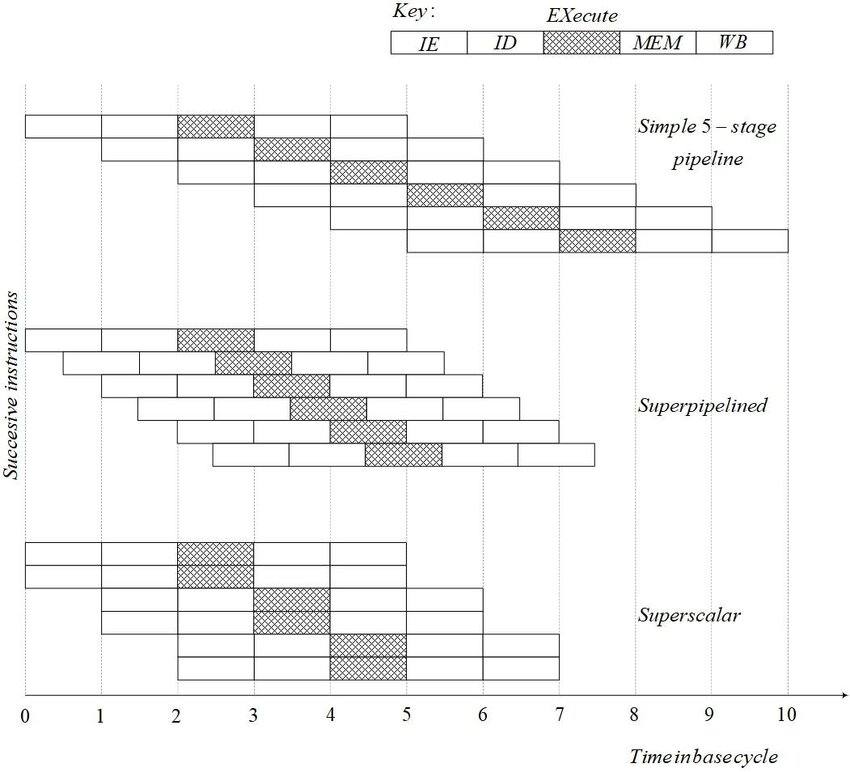
\includegraphics[width=0.5\textwidth]{SSvsSP.png}
  \caption{Superescalar contra Supersegmentado.}
\end{figure}

\subsection*{Limitaciones}

La aproximación superescalar depende de la habilidad para ejecutar múltiples instrucciones en paralelo. La expresión \textbf{paralelismo en las instrucciones} se refiere al grado en el que, en promedio, las instrucciones de un programa se pueden ejecutar en paralelo. Para maximizar el paralelismo en las instrucciones, se puede usar una combinación de optimizaciones realizadas por el compilador y de técnicas de hardware. Las principales limitaciones son:

\begin{itemize}
  \item \textbf{Dependencia de datos verdadera:} es cuando una instrucción necesita el dato producido por la primera instrucción. Si no hay dependencias, se puede captar y ejecutar dos instrucciones en paralelo. En caso de que exista esta dependencia de datos entre la primera y la segunda instrucción, se retrasa la segunda instrucción tantos ciclos de reloj como sea necesario para eliminar la dependencia.
  \item \textbf{Dependencia relativa al procedimiento:} la presencia de saltos en una secuencia de instrucciones complica el funcionamiento del cauce. Las instrucciones que siguen a una bifurcación tienen una dependencia relativa al procedimiento en ese bifurcación y no pueden ejecutarse hasta que se ejecute el salto.
  \item \textbf{Conflicto en los recursos:} Un conflicto en un recurso es una pugna de dos o más instrucciones por el mismo recurso al mismo tiempo. Desde el punto de vista del cauce segmentado, un conflicto en los recursos presenta el mismo comportamiento que una dependencia de datos. No obstante, hay algunas diferencias. Los conflictos en los recursos pueden superarse duplicando estos. Además, cuando una operación tarda mucho tiempo en finalizar, los conflictos en los recursos se pueden minimizar segmentando la unidad funcional apropiada.
  \item \textbf{Dependencia de salida.}
  \item \textbf{Antidependencia:} la restricción es similar a la de la dependencia verdadera pero a la inversa. En lugar e que la primera instrucción produzca un valor que usa la segunda instrucción, la segunda instrucción destruye un valor que utiliza la primera instrucción.
\end{itemize}

\subsection{Cuestiones relacionadas con el diseño}

\subsubsection*{Paralelismo en las instrucciones y paralelismo de la máquina}

El \textbf{paralelismo en las instrucciones} existe cuando las instrucciones de una secuencia son independientes y por tanto pueden ejecutarse en paralelo solapándose.

El paralelismo en las instrucciones depende de la frecuencia de dependencias de datos verdaderas y dependencias relativas al procedimiento que haya en el código. Estos factores dependen a su vez de la arquitectura del repertorio de instrucciones y de la aplicación.

El \textbf{paralelismo de la máquina} es una medida de la capacidad del procesador pra sacar partido al paralelismo en las instrucciones. El paralelismo de maquina depende del número de instrucciones que pueden captarse y ejecutarse al mismo tiempo y de la velocidad y sofisticación de los mecanismos que usa el procesador para localizar instrucciones independientes.

\subsubsection*{Políticas de emisión de instrucciones}

Se utiliza el término \textbf{emisión de instrucciones} para referirse al proceso de iniciar la ejecución de instrucciones en las unidades funcionales del procesador y el término \textbf{política de emisión de instrucciones} para referirse al protocolo usado para emitir instrucciones. 

El procesador intenta localizar instrucciones más allá del punto de ejecución en curso que puedan introducirse en el cauce y ejecutarse. Hay tres ordenaciones importantes:

\begin{itemize}
  \item El orden en que se captan las instrucciones.
  \item El orden en que se ejecutan las instrucciones.
  \item El orden en que las instrucciones actualizan los contenidos de los registros y de las posiciones de memoria.
\end{itemize}

Cuanto más sofisticado sea el procesador, menos limitado estará por la estrecha relación entre estas ordenaciones. Para optimizar la utilización de los diversos elementos del cauce, el procesador tendrá que alterar uno o más de estos órdenes con respecto al orden que se encontraría en una ejecución secuencial estricta. La única restricción que tiene el procesador es que el resultado debe ser correcto. De este modo, el procesador tiene que acomodar las diversas dependencias y conflictos discutido antes.

Podemos agrupar las políticas de emisión de instrucciones de los procesadores superescalares en las siguientes categorías:

\begin{itemize}
  \item \textbf{Emisión en orden y finalización en orden:} es la política de emisión más sencilla. Consiste en emitir instrucciones en el orden exacto en que lo haría una ejecución secuencial y escribir los resultados en ese mismo orden. Ni siquiera los cauces escalares siguen una política tan ingenua. No obstante, es útil considerar esta política como base con la cual comparar otras aproximaciones más sofisticadas.
  \item \textbf{Emisión en orden y finalización desordenada:} la finalización desordenada se usa en los procesadores RISC escalares para mejorar la velocidad de las instrucciones que necesitan ciclos. Con finalización desordenada, puede haber cualquier número de instrucciones en la etapa de ejecución en un momento dado, hasta alcanzar el máximo grado de paralelismo e la máquina ocupando todas la unidades funcionales. La emisión de instrucciones se para cuando hay una pugna por un recurso, una dependencia de datos o una dependencia relativa al procedimiento. Surge la \textbf{dependencia de salida}.
  \item \textbf{Emisión desordenada y finalización desordenada:} para permitir la emisión desordenada, es necesario desacoplar las etapas del cauce de decodificación y ejecución. Esto se hace mediante un buffer llamado \textbf{ventana de instrucciones}. Con esta organización, cuando un procesador termina de decodificar una instrucción, la coloca en la ventada de instrucciones. Mientras el buffer no se llene, el procesador puede continuar captando y decodificando nuevas instrucciones. Cuando una unidad funcional de la etapa de ejecución queda disponible, se puede emitir una instrucción desde la ventana de instrucciones a la etapa de ejecución. La única restricción es que el programa funcione correctamente. Por esta política surge el termino \textbf{antidependencia}.
\end{itemize}

\subsubsection*{Renombramiento de registros}

Cuando varias instrucciones compiten por el uso de los mismos registros, generando restricciones en el cauce que reducen las prestaciones. Un método para hacer frente a este tipo de conflictos de almacenamiento se basa en una solución tradicional para los conflictos en los recursos: la duplicación de recursos.

Con el \textbf{renombramiento de registros}, el hardware del procesador asigna dinámicamente los registros, que están asociados con los valores que necesitan las instrucciones en diversos instantes de tiempo. Cuando se crea un nuevo valor de registro, se asigna un nuevo registro para ese valor. Las instrucciones posteriores que accedan a ese valor como operando fuente en ese registro tienen que sufrir un proceso de renombramiento: las referencias a registros de esas instrucciones han de revisarse para referenciar el registro que contiene el valor que se necesita. 

\subsubsection*{Ejecución superescalar}

El proceso de captación de instrucciones, que incluye la predicción de saltos, se usa para formar un flujo dinámico de instrucciones. Se examinan las dependencias de este flujo, y el procesador puede eliminar las que sean artificiales. En esta ventana, las instrucciones ya no forman un flujo secuencial sino que están estructuradas de acuerdo a sus dependencias de dots verdaderas. El procesador lleva a cabo la etapa de ejecución de cada instrucción en un orden determinado por las dependencias de datos verdaderas y la disponibilidad de los recursos hardware. Por último, las instrucciones se vuelven a poner conceptualmente en un orden secuencial y sus resultados se almacenan.

\begin{figure}[H]
  \centering
  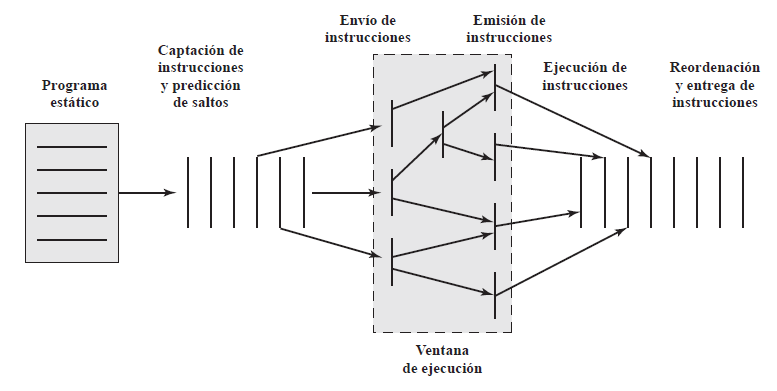
\includegraphics[width=0.7\textwidth]{ProcesamientoSE.png}
  \caption{Representación conceptual del procesamiento superescalar}
\end{figure}

\subsubsection*{Implementación superescalar}

\begin{itemize}
  \item Estrategias de captación simultánea de múltiples instrucciones.
  \item Lógica para determinar dependencias verdaderas entre valores de registros y mecanismos para comunicar esos valores.
  \item Mecanismos para iniciar o emitir múltiples instrucciones en paralelo.
  \item Recursos para la ejecución en paralelo de múltiples instrucciones.
  \item Mecanismos para entregar el estado del procesador en un orden correcto.
\end{itemize}

\subsubsection*{Consideraciones destacables en el procesamiento superescalar}

En el momento en que se produce una excepción hay varias instrucciones en ejecución. Si $I_1$ produce una excepción $\to$ ¿ha podido terminar $I_2$? $\to$ Estado inconsistente (excepciones imprecisas).

El comportamiento debería ser idéntico al que tendría la misma computadora no segmentada. Para garantizar un estado consistente:

\begin{itemize}
  \item Instrucciones anteriores terminan correctamente.
  \item La que origina la excepción y siguientes se abortan.
  \item Tras la rutina de tratamiento se comienza por la que originó la excepción.
\end{itemize}

\subsection{Pentium 4}

Aunque el concepto de diseño superescalar se asocia generalmente con la arquitectura RISC, se pueden aplicar los mismos principios superescalares a una máquina CISC.\@ El ejemplo más notable de ello tal vez sea el Pentium.

\begin{figure}[H]
  \centering
  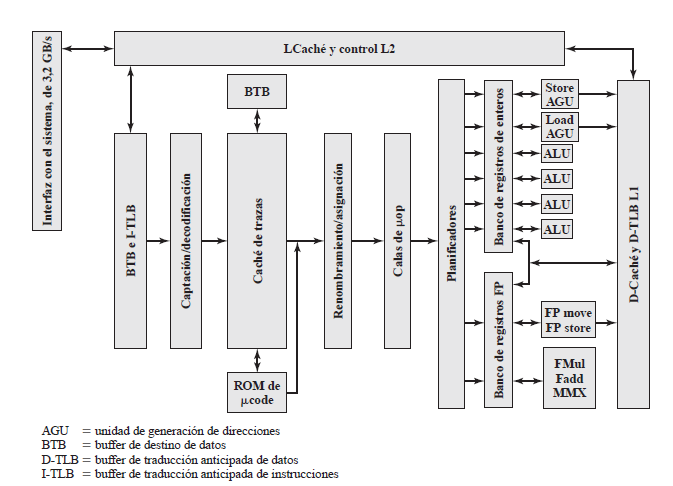
\includegraphics[width=0.6\textwidth]{Pentium4.png}
  \caption{Diagrama de bloques del Pentium 4}
\end{figure}

El funcionamiento del Pentium 4 se puede resumir como sigue:

\begin{itemize}
  \item El procesador capta instrucciones de memoria en el orden en que aparecen en el programa estático.
  \item Cada instrucción se traduce en una o más instrucciones RISC de tamaño fijo conocidas como \textbf{microoperaciones} o \textbf{micro-ops}.
  \item El procesador ejecuta las micro-ops en una organización de cauce superescalar, de modo se pueden ejecutar desordenadas.
  \item El procesador entrega los resultados de la ejecución de cada micro-op al conjunto de registros, en el orden del flujo del programa original.
\end{itemize}

En realidad, la arquitectura del Pentium 4 consta de una envoltura CISC con un núcleo RISC interno. Las micro-ops RISC internas pasan a través de un cauce con al menos veinte etapas; en algunos casos, las micro-ops necesitan múltiples etapas de ejecución, lo que se traduce en un cauce aún más largo.

\subsection{Arquitectura IA-64}

Intel se asocia con HP para desarrollar una nueva arquitectura de 64 bits, llamada IA-64. La arquitectura IA-64 no es una ampliación a 64 bits de la arquitectura de 32 bits x86 de Intel. La IA-64 aprovecha la enorme circuitería y la gran velocidad disponibles en las más recientes generaciones de microchips gracias a la utilización sistemática del paralelismo.

\subsubsection{Motivación}

Los conceptos básicos en los que se fundamenta la arquitectura IA-64 son los siguientes:

\begin{itemize}
  \item Paralelismo en las instrucciones que queda explícito en las instrucciones máquina, en lugar de depender del procesador en tiempo de ejecución.
  \item Palabras de instrucción largas o muy largas (LIW\footnote[1]{long instruction word}/VLIW\footnote[2]{very long instruction word}).
  \item Ejecución de saltos basada en predicados (concepto diferente al de predicción de saltos).
  \item Carga especulativa.
\end{itemize}

Intel y HP hacen referencia a esta combinación de conceptos con el nombre de computación con instrucciones explícitamente paralelas (EPIC). La arquitectura IA-64 consiste en un repertorio de instrucciones real destinado a ser implementado usando la tecnología EPIC.\@ El primer producto de Intel basado en IA-64 es conocido con el nombre de \textbf{Itanium}.

\begin{table}[h]
\centering
\begin{tblr}{
  width = \linewidth,
  colspec = {Q[462]Q[479]},
  row{1} = {c},
  hlines,
  vlines,
}
\textbf{Superescalar}                                                                                          & \textbf{IA-64}                                                                                                            \\
Instrucciones de tipo RISC, una por palabra                                                                    & Instrucciones de tipo RISC puestas en grupos de tres                                                                      \\
Multiples unidades de ejecución en paralelo                                                                    & Múltiples unidades de ejecución en paralelo                                                                               \\
Reordena y optimiza el flujo de instrucciones en tiempo de ejecución                                           & Reordena y optimiza el flujo de instrucciones en tiempo de compilación.                                                   \\
Predicción de saltos con ejecución especulativa de un camino.                                                  & Ejecución especulativa de los dos caminos de una bifurcación.                                                             \\
{Carga de datos desde memoria solo cuando es necesario, e intenta encontrar los datos primero en las cachés.} & {Carga datos especulativamente antes de que se necesiten, y sigue intentando encontrar los datos primero en las cachés.} 
\end{tblr}
\end{table}

Intel y HP han propuesto un planteamiento de diseño global que permite la utilización eficaz de un procesador con muchas unidades de ejecución en paralelos. El corazón de este nuevo enfoque es el concepto de paralelismo explícito. En esta aproximación, el compilador planifica estáticamente las instrucciones en tiempo de compilación, en lugar de que lo haga dinámicamente el procesador en tiempo de ejecución. El compilador determina qué instrucciones pueden ejecutarse en paralelo e incluye esta información en la instrucción máquina. El procesador usa esa información para llevar a cabo la ejecución paralela. Una ventaja de esta aproximación es que el procesador EPIC no requiere tanta circuitería compleja como un procesador superescalar capaz de ejecutar instrucciones sin orden. Además, mientras que el procesador tiene que determinar la posibilidad de una potencial ejecución en paralelo en cuestión de nanosegundos, el compilador dispone de un plazo varios órdenes de magnitud mayor para examinar el código con detenimiento y estudiar el programa globalmente.

\subsubsection{Organización general}

Como cualquier arquitectura de procesador, la IA-64 puede implementarse con diversas organizaciones. Sus características más importantes son:

\begin{itemize}
  \item \textbf{Gran numero de registros:} el formato de instrucción de la arquitectura IA-64 supone el empleo de 256 registros, 126 registros de 64 de uso general para uso con enteros, con datos lógicos y para propósito general, y 128 registros de 82 bits para su uso con coma flotante y gráficos. También hay 64 bits de predicado de un bit, usados para la ejecución con predicados.
  \item \textbf{Multiples unidades de ejecución:} una máquina superescalar típica puede tener cuatro cauces paralelos, empleando cuatro unidades de ejecución en paralelo tanto para la parte de enteros del procesador como para la parte de la coma flotantes. Se espera que la IA-64 se implemente en sistemas con ocho o más unidades paralelas.
\end{itemize}

En la arquitectura IA-64 se definen cuatro tipos de unidades de ejecución:

\begin{itemize}
  \item \textbf{I:} para instrucciones aritméticas con enteros, de desplazamiento y suma, lógicas de comparación y multimedia con enteros.
  \item \textbf{M:} cargas y almacenamientos entre registros y memoria más algunas operaciones de la ALU con enteros.
  \item \textbf{B:} instrucciones de salto.
  \item \textbf{F:} instrucciones de coma flotante.
\end{itemize}

\subsubsection*{Formato de instrucción}

La arquitectura IA-64 define un \textbf{paquete} de 128 bits que contiene tres instrucciones, llamadas \textbf{silabas}, y un campo plantilla. El procesador puede captar uno o más paquetes de instrucciones a la vez; y cada captación indica qué instrucciones se pueden ejecutar en paralelo. La interpretación de este campo no se limita a un único paquete. Por el contrario, el procesador puede examinar varios paquetes para determinar qué instrucciones pueden ejecutarse en paralelo. 

Las instrucciones agrupadas no tienen que estar en el orden original del programa. Además, debido a la flexibilidad del campo plantilla, el compilador puede mezclas instrucciones dependientes e independientes en el mismo paquete.

\begin{figure}[h]
  \centering
  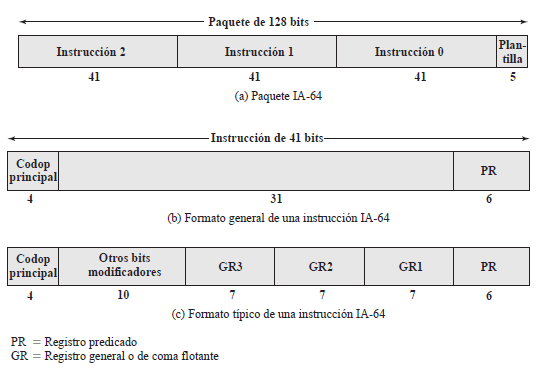
\includegraphics[width=0.6\textwidth]{InstruccionesIA-64.png}
  \caption{Formato de instrucción de la arquitectura IA-64}
\end{figure}

El valor de plantilla tiene dos propósitos:

\begin{itemize}
  \item El campo especifica la correspondencia de las instrucciones con los tipos de unidades de ejecución. No son posibles todas las correspondencias de instrucciones con unidades.
  \item El campó indica la presencia de posibles \textbf{paradas}. Una parada indica al hardware que una o más instrucciones anteriores a la parada pueden tener ciertos tipos de dependencias de recursos con una o más instrucciones posteriores a la parada.
\end{itemize}

\subsubsection*{Saltos predicados}

Los saltos predicados son una técnica de compilación. El compilador elimina saltos del programa usando ejecución condicional, es necesario soporte de hardware. Se deja que ambas ramas de un salto condicional se ejecuten en paralelo.
\section{Procesamiento paralelo}

\subsection{Organizaciones con varios procesadores}

\subsubsection*{Tipos de sistemas paralelos}

La taxonomia introducida por Flynn es todavía la forma más común de clasificar a los sistemas según sus capacidades de procesamiento paralelo. Flynn propuso las siguientes categorías o clases de computadoras:

\begin{itemize}
  \item \textbf{Single Instruction Single Data (SISD):} un único procesador interpreta una única secuencia de instrucciones para operar con los datos almacenados en una única memoria. Los computadores monoprocesador caen dentro de esta categoría.
  \item \textbf{Single Instruction Multiple Data (SIMD):} una única máquina controla paso a paso la ejecución simultánea y sincronizada de un cierto número de elementos de proceso. Cada elemento de proceso tiene una memoria asociada, de forma que cada instrucción es ejecutada por cada procesador con un conjunto de datos diferentes. Los procesadores vectoriales y los matriciales pertenecen a esta categoría.
  \item \textbf{Multiple Instruction Single Data (MISD):} se transmite una secuencia de datos a un conjunto de procesadores, cada uno de los cuales ejecuta una secuencia de instrucciones diferente. Esta estructura nunca ha sido implementada.
  \item \textbf{Multiple Instruction Multiple Data (MIMD):} un conjunto de procesadores ejecuta simultáneamente secuencias de instrucciones diferentes con conjuntos de datos diferentes. Los SMP, los \textit{clusters} y los sistemas NUMA son ejemplos de esta categoría.
\end{itemize}

En la organización MIMD los procesadores son de uso general; cada uno es capaz de procesar todas las instrucciones necesarias para realizar las transformaciones apropiadas de los datos. Los computadores MIMD se pueden subdividir además según la forma que tienen los procesadores para comunicarse. Si los procesadores comparten una memoria común, entonces cada procesador accede a los programas y datos almacenados en la memoria compartida, y los procesadores se comunican unos con otros a través de esa memoria. La forma más común de este tipo de sistema se conoce como \textbf{multiprocesador simétrico (SMP)}. En un SMP, varios procesadores comparten una única memoria mediante un bus compartido u otro tipo de mecanismo de interconexión. Una característica distintiva de estos sistemas es que el tiempo de acceso a memoria principal es aproximadamente el mismo para cualquier procesador. Un desarrollo más reciente es la organización con \textbf{acceso no uniforme a memoria (NUMA)}. Como el propio nombre indica, el tiempo de acceso a zonas de memoria diferentes puede diferir en un computador NUMA.\@

Un conjunto de computadores monoprocesador independientes o de SMP pueden interconectarse para formar un \textit{cluster}. La comunicación entre los computadores se realiza mediante conexiones fijas o mediante algún tipo de red.



\appendix

\end{document}
